We present here more details on the experimental protocol used in the main
paper as well as new experiments.
\subsection{Alternative hyperparameters sampling}\label{subsection:sampling}
Many quadrature rules such as \ac{MC} and \ac{QMC} methods are well suited for
\acl{ITL}. For instance when $\hyperparameterspace$ is high dimensional,
\ac{MC} is typically prefered over \ac{QMC}, and vice versa. If
$\hyperparameterspace$ is one dimensional and the function to integrate is
smooth enough then a Gauss-Legendre quadrature would be preferable. In
\cref{sec:V} of the main paper we provide a unified notation to handle
\ac{MC}, \ac{QMC} and other quadrature rules. In the case of
\begin{itemize}
    \item \ac{MC}: $w_j = \frac{1}{m}$ and $(\theta_j)_{j=1}^m
    \sim \mu^{\otimes m}$.
    %Note that if $\mu=\delta_{\theta_j'}$ is a dirac measure  centered at
    %$\theta_{j'}$ then $\theta_j=\theta_j'$.
    \item \ac{QMC}: $w_j = m^{-1}F^{-1}(\theta_j)$ and $(\theta_j)_{j=1}^m$
    is a sequence with values in $[0, 1]^d$ such as the % uniform properties
    Sobol or Halton sequence, $\mu$ is assumed to be absolutely continuous
    \acs{wrt} the Lebesgue measure, $F$ is the associated cdf.
    \item Quadrature rules: $((\theta_j, w'_j))_{j=1}^m$ is the indexed set of
    locations and weights produced by the quadrature rule, $w_j
    = w'_j f_{\mu}(\theta_j)$, $\mu$ is assumed to be absolutely continuous
    \acs{wrt} the Lebesgue measure, and $f_\mu$ denotes its corresponding
    probability density function.
\end{itemize}
\subsection{Impact of the number of hyperparameters sampled}
\begin{figure}[!htbp]
    \centering
    \includegraphics[width=\textwidth]{src/fig/autogen/iqr_m.pdf}
    \caption{Impact of the number of hyperparameters sampled.
             \label{figure:iqr_m}}
\end{figure}
In the experiment presented on \cref{figure:iqr_m}, on the sine synthetic
benchmark, we draw $n=1000$ training points and study the impact of increasing
$m$ on the quality of the quantiles at $\theta\in\Set{0.05, 0.25, 0.5, 0.75,
0.95}$. We notice that when $m\ge34\approx\sqrt{1000}$ there is little benefit
to draw more $m$ samples are the quantile curves do not change on the
$n_{\text{test}}=2000$ test points.
\subsection{Smoothifying the cost function} \label{subsection:infimal_convo}
The resulting $\kappa$-smoothed ($\kappa\in\reals_+$) absolute value
($\psi_{1}^\kappa$) and positive part ($\psi_{+}^\kappa$) are as follows:
\begin{align*}
  \psi_{1}^\kappa(p) &\defeq \left(\kappa \abs{\cdot} \square \frac{1}{2}
    \abs{\cdot}^2 \right)(p)
     =
     \begin{cases}
        \frac{1}{2\kappa}p^2 & \text{if $\abs{p} \le \kappa$} \\
        \abs{p} - \frac{\kappa}{2} & \text{otherwise},
    \end{cases}\\
     \psi_{+}^\kappa(p) &\defeq \left(\kappa\abs{\cdot}_+ \square\frac{1}{2}
     \abs{\cdot}^2 \right)(p) =
     \begin{cases}
         \frac{1}{2\kappa}\abs{p}_+^2 & \text{if $p \le \kappa$} \\
         p - \frac{\kappa}{2} & \text{otherwise.}
     \end{cases}
\end{align*}
where $\square$ is the classical infimal convolution \citep{bauschke2011convex}.
All the smoothified loss functions used in this paper
have been gathered in \cref{table:integrated_risks}.
\paragraph{Remarks}
\begin{itemize}[labelindent=0cm,leftmargin=*,topsep=0cm,partopsep=0cm,
                parsep=0cm,itemsep=0cm]
    \item Minimizing the $\kappa$-smoothed pinball loss
    \begin{align*}
     \parametrizedcost{\hyperparameter,\kappa}(y, h(x))=\abs{\hyperparameter -
     \indicator{\reals_{-}}(y - h(x))}\psi_1^\kappa(y - h(x)),
    \end{align*}
    yields the quantiles when $\kappa\rightarrow 0$, the expectiles as
    $\kappa\to+\infty$. The intermediate values are known as M-quantiles
    \citep{breckling1988m}.
    \item In practice, the absolute value and positive part can be approximated
    by a smooth function by setting the smoothing parameter $\kappa$ to be a
    small positive value;
    % \rb{or even zero}
    the optimization showed a robust behaviour \acs{wrt} this choice with a
    random coefficient initialization.
    % \rb{as    pointed out by \citet{lewis2013nonsmooth}}.
%     \item the cost of evaluating the model $h$ one $n$ samples and $m$
%     hyperparameters is $\mathcal{O}(n^2m + m^2n)$ and it takes
%     $\mathcal{O}(m^2+n^2)$ to fit in memory.
\end{itemize}\par
\paragraph{Impact of the Huber loss support}
The influence of the $\kappa$ parameter is illustrated in
\cref{figure:kappa_study}.  For this experiment, $10000$ samples have been
generated from the sine wave dataset described in \cref{paragraph:datasets},
and the model have been trained on $100$ quantiles generated from a
Gauss-Legendre Quadrature.  When $\kappa$ is large the expectiles are learnt
(dashed lines) while when $\kappa$ is small the quantiles are recovered (the
dashed lines on the right plot match the theoretical quantiles in plain lines).
It took $225$s ($258$ iteration, and $289$ function evaluations) to train
for $\kappa=1\cdot 10^1$, $1313$s for $\kappa=1\cdot 10^{-1}$ ($1438$
iterations and $1571$ function evaluations), $931$s for $\kappa=1e^{-3}$
($1169$ iterations and $1271$ function evaluations) and $879$s for $\kappa=0$
($1125$ iterations and $1207$ function evaluations). We used a GPU Tensorflow
implementation and run the experiments in float64 on a computer equipped with a
GTX $1070$, and intel i7 $7700$ and $16$GB of DRAM.
\begin{figure}[!htbp]
    \centering
    \resizebox{!}{.5\linewidth}{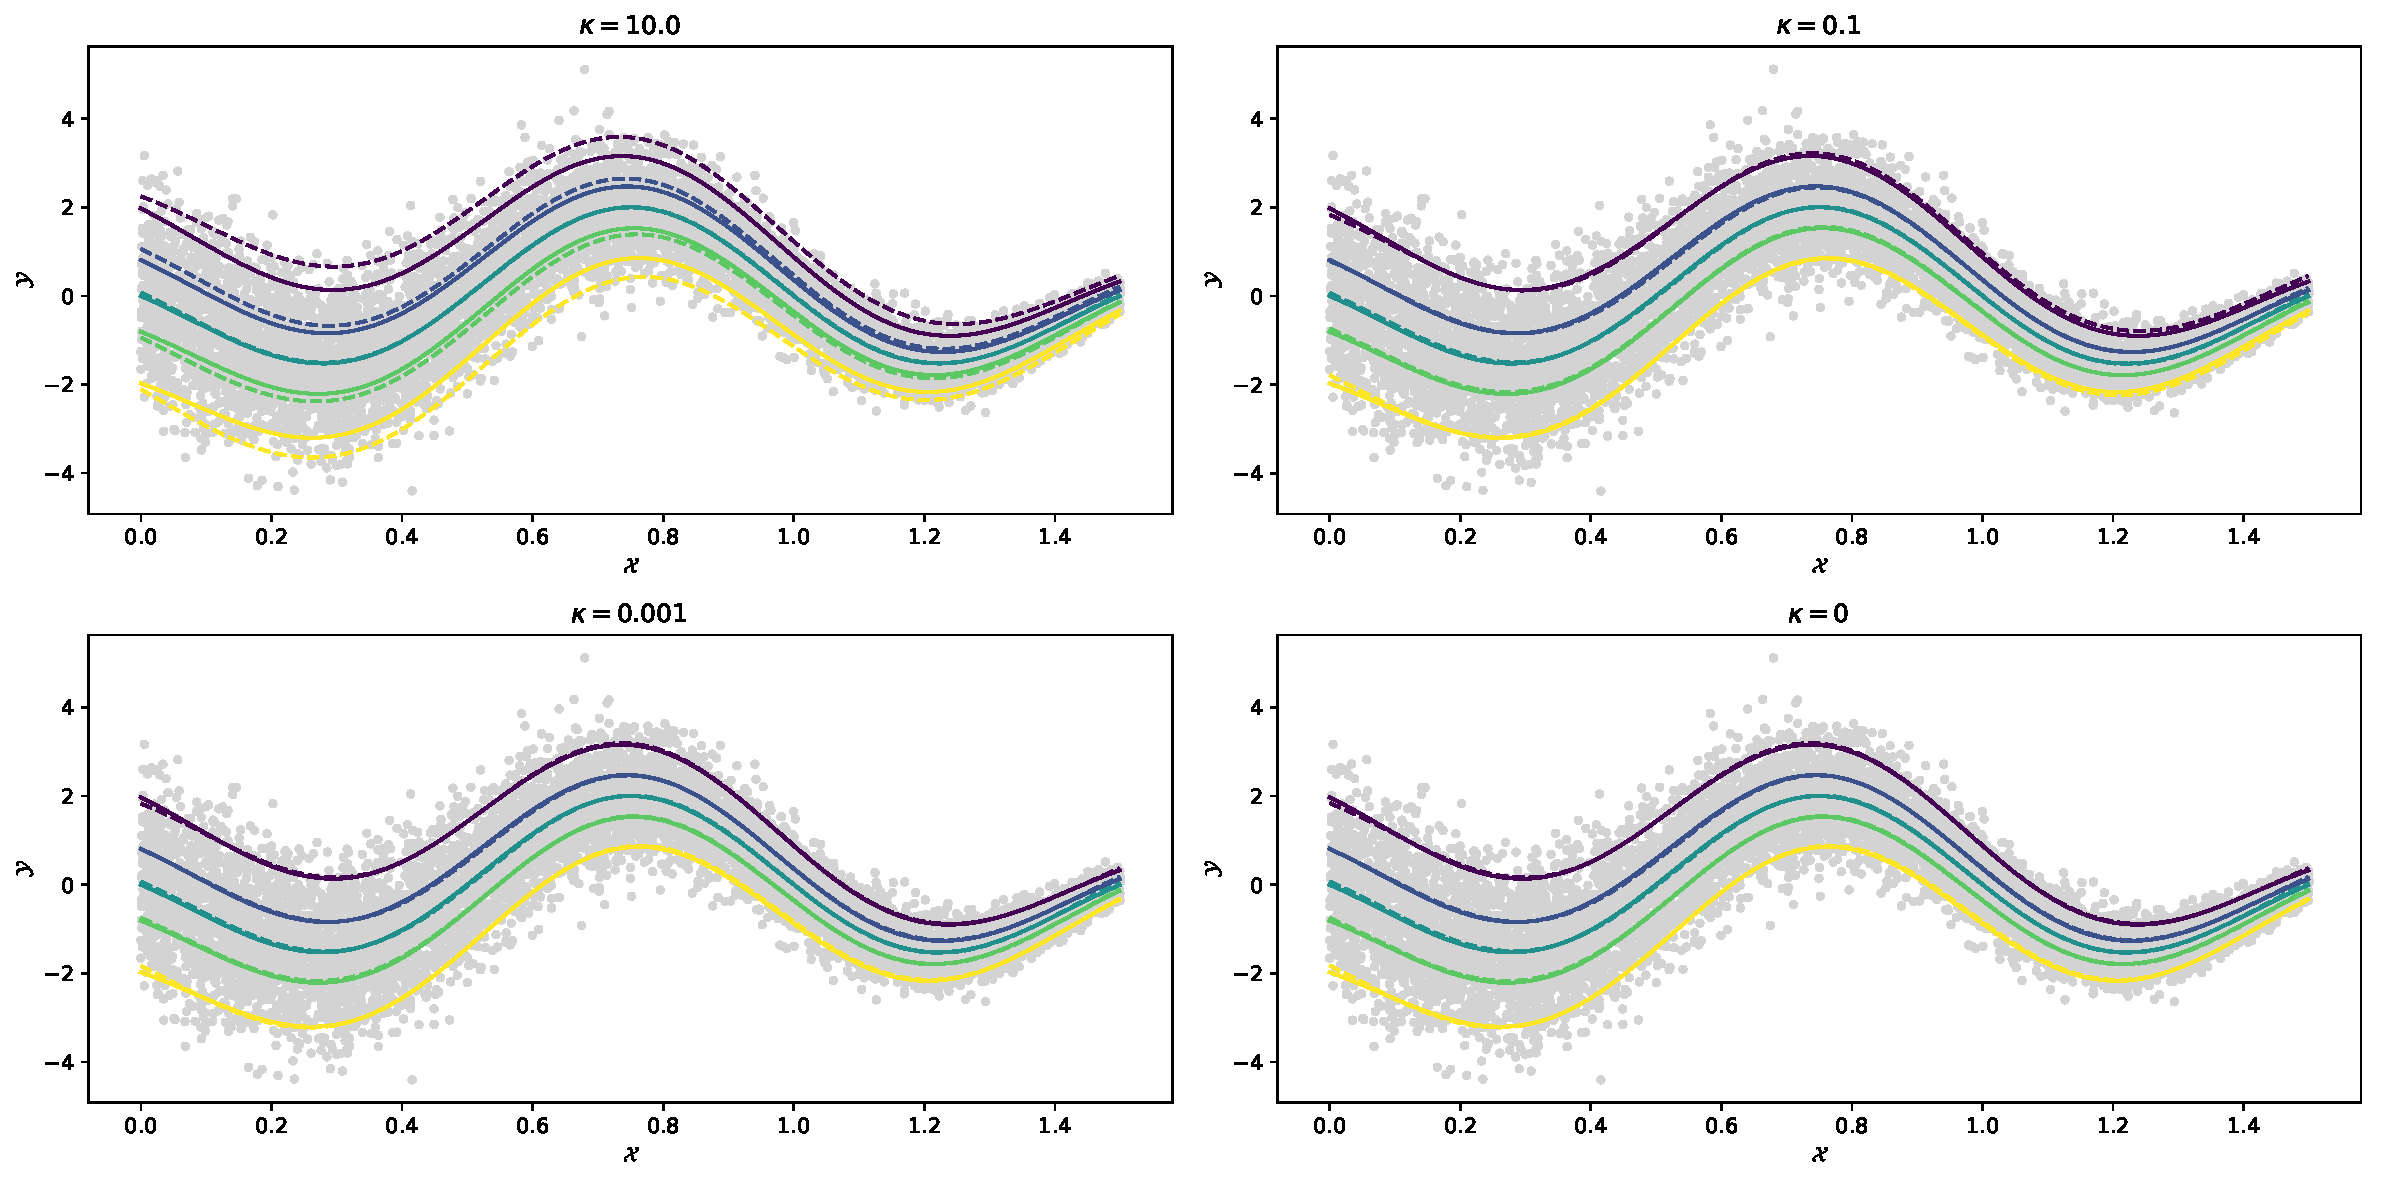
\includegraphics{src/fig/autogen/iqr_kappa.pdf}}
    \caption{Impact of the Huber loss smoothing of the pinball loss for
    differents values of $\kappa$. \label{figure:kappa_study}}
\end{figure}
\begin{table}[tb]
    \caption{Examples for objective \eqref{equation:integrated_cost}.
    $\psi_1^\kappa$, $\psi_+^\kappa$: $\kappa$-smoothed absolute value
    and positive part. $h_{x}(\hyperparameter)\defeq h(x)(\theta)$.
    \label{table:integrated_risks}}
    \begin{center}
      \addtolength{\tabcolsep}{-3pt}
      \renewcommand{\arraystretch}{0.8}
        \begin{tiny}
            \begin{sc}
                \resizebox{\textwidth}{!}{%
                \begin{tabular}{lll}
                    \toprule
                    & loss & penalty \\
                    \midrule
                    Quantile  & $\displaystyle\int_{\closedinterval{0}{1}}
                    \abs{\hyperparameter - \indicator{\reals_{-}}(y -
                    h_x(\hyperparameter))}\abs{y - h_x(\hyperparameter)}
                    d\mu(\hyperparameter)$ &
                    $\lambda_{nc}\int_{\closedinterval{0}{1}}
                    \abs{-\frac{dh_x}{d\hyperparameter}(\hyperparameter)}_+
                    d\mu(\hyperparameter) +
                    \frac{\lambda}{2}\norm{h}_{\mcH_K}^2$ \\
                    M-Quantile (smooth)  &
                    $\displaystyle\int_{\closedinterval{0}{1}}
                    \abs{\hyperparameter - \indicator{\reals_{-}}(y -
                    h_x(\hyperparameter))}\psi_1^\kappa\left(y -
                    h_x(\hyperparameter)\right)d\mu(\hyperparameter)$ &
                    $\lambda_{nc}\int_{(0, 1)} \psi_+^\kappa\left(-
                    \frac{dh_x}{d\hyperparameter}(\hyperparameter)\right)
                    d\mu(\hyperparameter) +
                    \frac{\lambda}{2}\norm{h}_{\mcH_K}^2$ \\
                    Expectiles (smooth) &
                    $\displaystyle\int_{\closedinterval{0}{1}}
                    \abs{\hyperparameter - \indicator{\reals_{-}}(y -
                    h_x(\hyperparameter))}\left(y -
                    h_x(\hyperparameter)\right)^2d\mu(\hyperparameter)$ &
                    $\lambda_{nc} \int_{(0, 1)}
                    \abs{-\frac{dh_x}{d\hyperparameter}(\hyperparameter)}_+^2
                    d\mu(\hyperparameter) +
                    \frac{\lambda}{2}\norm{h}_{\mcH_K}^2$ \\
                    Cost-Sensitive & $\displaystyle\int_{
                    \closedinterval{-1}{1}} \abs{\frac{\hyperparameter + 1}{2}
                    - \indicator{\{-1\}}(y)}\abs{1 -
                    yh_{x}(\hyperparameter)}_{+} d\mu(\theta)$ & $
                    \frac{\lambda}{2}\norm{h}_{\mcH_K}^2$ \\
                    Cost-Sensitive (smooth) &
                    $\displaystyle\int_{\closedinterval{-1}{1}}
                    \abs{\frac{\hyperparameter + 1}{2} -
                    \indicator{\{-1\}}(y)}\psi_+^\kappa\left(1 -
                    yh_{x}(\hyperparameter)\right) d\mu(\theta)$ & $
                    \frac{\lambda}{2}\norm{h}_{\mcH_K}^2$ \\
                    Level-Set   &
                    $\displaystyle\int_{\closedinterval{\epsilon}{1}}
                    -t(\hyperparameter) +
                    \frac{1}{\theta}\abs{t(\hyperparameter) -
                    h_x(\hyperparameter)}_+
                    d\mu(\hyperparameter)$ & $
                    \frac{1}{2}\displaystyle\int_{
                    \closedinterval{\epsilon}{1}}
                    \norm{h(\cdot)(\hyperparameter)}_{
                    \mcH_{k_{\inputspace}}}^2 d\mu(\hyperparameter) +
                    \frac{\lambda}{2}\norm{t}_{\mcH_{k_b}}^2$\\ \bottomrule
                \end{tabular}}
            \end{sc}
        \end{tiny}
        \addtolength{\tabcolsep}{3pt}
        \renewcommand{\arraystretch}{0.8}
    \end{center}
\end{table}
%
\subsection{Experimental protocol for \ac{QR}}  \label{subsection:proto_exp} In
this section, we give additional details regarding the choices being made while
implementing the \ac{ITL} method for $\infty$-\ac{QR}.
%
%\paragraph{Crossing Quantiles}
%The model was trained with a
%bias.  For $k_{\inputspace}$ a Gaussian kernel was used,
%$k_{\hyperparameterspace}$ and $k_{b}$ were Laplacian kernels. All bandwidths
%were set to $10$ to emphasise the possible crossings.

%\begin{dmath}\label{equation:non_crossing_constraint}
    %\Omega(h) = \lambda_{c}\sum_{i=1}^N \int_{(0, 1)} \abs{
    %-\frac{\partial}{\partial \tau} h_{\tau}(X_i)}_+ d\mu(\tau) +
    %\frac{\lambda}{2}(\norm{f}_{K}^2 + \norm{b}_{kb}^2).
%\end{dmath}
%Note that if the integral in \cref{equation:non_crossing_constraint} in uses
%the same samples $\tau_j$'s as the one used to approximate the cost function
%$\cost$, then the representer theorem applies with the expansion given in
%\cref{equation:expanded_non_crossing_constraint}.
%\begin{dmath}\label{equation:expanded_non_crossing_constraint}
    %\Omega_\lambda(h)=\lambda\sum_{j=1}^T\sum_{i=1}^N \abs{-\sum_{j'=1}^T
    %\sum_{i'=1}^N\alpha_{i'j'} k_{\inputspace}(x_i, x_{i'})\frac{\partial
    %k_{\hyperparameterspace}}{\partial\tau_j}(\tau_j, \tau_{j'}) -
    %\beta_j\frac{\partial k_b}{\partial \tau_j}(\tau_j, \tau_{j'})}_+ +
    %\sum_{i, i'=1}^N\sum_{j,
    %j'=1}^T\alpha_{ij}\alpha_{i'j'}k_{\inputspace}(x_i,
    %x_{i'})k_{\hyperparameterspace}(\tau_j,
    %\tau_{j'})+\beta_{j}\beta_{j'}k_b(\tau_j, \tau_{j'}).
%\end{dmath}
%\begin{center}
    %\begin{figure}[h]
        %% \resizebox{!}{.65\linewidth}{\includegraphics{fig/bias_experiment.eps}}
        %\caption{Model misspecification in quantile regression on the dataset
        %Engel. Left plot shows a linear model with bias and right plot without
        %bias.\label{figure:misspecified_models}}
    %\end{figure}
%\end{center}
%\par
%
\paragraph{\ac{QR} real datasets}
%
For $\infty$-\ac{QR}, $k_{\inputspace}$, $k_{\hyperparameterspace}$ were
Gaussian kernels. We set a bias term $k_b=k_{\hyperparameterspace}$. The
hyperparameters optimized were $\lambda$, the weight of the ridge penalty,
$\sigma_\inputspace$, the input kernel parameter, and
$\sigma_\hyperparameterspace=\sigma_b$, the output kernel parameter. They were
optimized in the (log)space of $\closedinterval{10^{-6}}{10^{6}}^3$. The
non-crossing constraint $\lambda_{nc}$ was set to $1$. The model was trained on
the continuum $\Theta=\openinterval{0}{1}$ using QMC and Sobol sequences. For
all datasets we draw $m=100$ quantiles form a Sobol sequence \par
%
For \ac{JQR} we similarly chose two Gaussian kernels. The optimized
hyperparameters were the same as for $\infty$-\ac{QR}.
% are also the bandwidth of the Gaussian kernel acting on the inputs, the bandwith
% of the kernel acting on the outputs, and the regularization tradeoff $\lambda$
% which where optimized in the (log)space $\closedinterval{10^{-6}}{10^{6}}^3$.
The quantiles learned were $\theta\in\Set{0.1, 0.3, 0.5, 0.7, 0.9}$.

For the IND-\ac{QR} baseline, we trained independently a non-paramatric
quantile estimator as described in \citet{takeuchi2006nonparametric}. A
Gaussian kernel was used and its bandwidth was optimized in the (log)space of
$\closedinterval{10^{-6}}{10^6}$. No non-crossing was enforced. \par
%
% \paragraph{Impact of the $\mcH_{k_{\hyperparameterspace}}$ kernel}
% See \cref{figure:gamma_t_study}.
% \begin{center}
%     \begin{figure}
%         % \resizebox{!}{.5\linewidth}{\includegraphics{fig/gamma_t_study.eps}}
%         \caption{Impact of the hyperparameter $\gamma_{\tau}$ on the
%         hyperparameter kernel $k_{\hyperparameterspace}$. Top row shows models
%         with a bias terms for $\gamma_{\tau}\in\Set{0.1, 100}$
%         respectfully left to right.  Bottom row shows the same for models
%         without bias.}
%     \label{figure:gamma_t_study}
%     \end{figure}
% \end{center}
\subsection{Experiments with \ac{CSC}}
\label{subsection:csc_expe}
In this section we provide numerical illustration concerning the \ac{CSC} problem.
We used the Iris \acs{UCI} dataset with $4$ attributes and $150$
samples, the two synthetic \textsc{scikit-learn}
\citep{pedregosa2011scikit} datasets \textsc{Two-Moons} (noise=$0.4$) and
$\textsc{Circles}$ (noise=$0.1$) with both $2$ attributes and $1000$
samples and a third synthetic \textsc{scikit-learn} dataset \textsc{Toy}
(class sep=$0.5$) with $20$ features ($4$ redundant and $10$ informative)
and $n=1000$ samples.\par
%
As detailed in \cref{section:infinite_tasks}, \acl{CSC} on a continuum
$\hyperparameterspace = \closedinterval{-1}{1}$ that we call \ac{ICSC}
can be tackled by our proposed technique.  In this case, the hyperparameter
$\hyperparameter$ controls the tradeoff between the importance of the correct
classification with labels $-1$ and $+1$. When $\hyperparameter = -1$,
class $-1$ is emphasized; the probability of correctly classified instances
with this label (called specificity) is desired to be $1$.  Similarly, for
$\hyperparameter = +1$, the probability of correct classification of samples
with label $+1$ (called sensitivity) is ideally $1$.\par
%
To illustrate the advantage of (infinite) joint learning we used two synthetic
datasets \textsc{Circles} and \textsc{Two-Moons} and the \acs{UCI}
\textsc{Iris} dataset. We chose $k_{\inputspace}$ to be a Gaussian kernel with
bandwidth $\sigma_{\inputspace}=(2\gamma_{\inputspace})^{(-1/2)}$ the median of
the Euclidean pairwise distances of the input points \citep{jaakkola1999using}.
$k_{\hyperparameterspace}$ is also a Gaussian kernel with bandwidth
$\gamma_{\hyperparameterspace}=5$.  We used $m=20$ for all datasets.
%
As a baseline we trained independently 3 \acl{CSC} classifiers with
$\hyperparameter\in\Set{-0.9,0, 0.9}$. We repeated $50$ times a random $50-50\%$
train-test split of the dataset and report the average test error and standard
deviation (in terms of sensitivity and specificity) \par
%
Our results are illustrated in \cref{table:csc_results}. For $\theta=-0.9$, both
 independent and joint learners give the desired $100\%$ specificity; the
joint \acl{CSC} scheme however has significantly higher sensitivity value
($15\%$ vs $0\%$) on the dataset \textsc{Circles}. Similar conclusion holds for the
$\theta=+0.9$ extreme: the ideal sensitivity is reached by both techniques, but
the joint learning scheme performs better in terms of specificity ($0\%$ vs
$12\%$) on the dataset \textsc{Circles}. \par
%
\begin{table*}[!htbp]
    \caption{\acs{ICSC} vs Independent (IND)-\acs{CSC}. Higher is
    better.\label{table:csc_results}}
    \addtolength{\tabcolsep}{-3pt}
    \renewcommand{\arraystretch}{0.8}% Tighter
    \begin{center}
        \begin{tiny}
            \begin{sc}
                \resizebox{.7\textwidth}{!}{%
                \begin{tabular}{cccccccc}
                    \toprule
                    \multirow{2}{*}{Dataset} & \multirow{2}{*}{Method} &
                    \multicolumn{2}{c}{$\theta=-0.9$} &
                    \multicolumn{2}{c}{$\theta=0$} &
                    \multicolumn{2}{c}{$\theta=+0.9$} \\
                    \cmidrule(lr){3-4} \cmidrule(lr){5-6} \cmidrule(lr){7-8} &
                    & \textsc{sensitivity} & \textsc{specificity} &
                    \textsc{sensitivity} & \textsc{specificity} &
                    \textsc{sensitivity} & \textsc{specificity} \\
                    \midrule
                    \multirow{ 2}{*}{\textsc{Two-Moons}} & IND &
                    $0.3\pm0.05$ & $0.99\pm0.01$ & $0.83\pm0.03$ &
                    $0.86\pm0.03$ & $0.99\pm0$ & $0.32\pm0.06$ \\
                                                & \acs{ICSC} & $0.32\pm0.05$ &
                    $0.99\pm0.01$ & $0.84\pm0.03$ & $0.87\pm0.03$ & $1\pm0$ &
                    $0.36\pm0.04$  \\
                    \multirow{ 2}{*}{\textsc{Circles}} & IND & $0\pm0$
                    & $1\pm0$ & $0.82\pm0.02$ & $0.84\pm0.03$ & $1\pm0$ &
                    $0\pm0$ \\
                                              & \acs{ICSC} & $0.15\pm0.05$ &
                    $1\pm0$ & $0.82\pm0.02$ & $0.84\pm0.03$ & $1\pm0$ &
                    $0.12\pm0.05$  \\
                    \multirow{ 2}{*}{\textsc{Iris}} & IND &
                    $0.88\pm0.08$ & $ 0.94\pm0.06$ & $0.94\pm0.05$ &
                    $0.92\pm0.06$ & $0.97\pm0.05$ & $0.87\pm0.06$\\
                                           & \acs{ICSC} & $0.89\pm0.08$ &
                    $0.94\pm0.05$ & $0.94\pm0.06$ & $0.92\pm0.05$ &
                    $0.97\pm0.04$ & $0.90\pm0.05$
                    \\
                    \multirow{ 2}{*}{\textsc{Toy}} & IND &
                    $0.51\pm0.06$ & $ 0.98\pm0.01$ & $0.83\pm0.03$ &
                    $0.86\pm0.03$ & $0.97\pm0.01$ & $0.49\pm0.07$\\
                                           & \acs{ICSC} & $0.63\pm0.04$ &
                    $0.96\pm0.01$ & $0.83\pm0.03$ & $0.85\pm0.03$ &
                    $0.95\pm0.02$ & $0.61\pm0.04$
                    \\
                    \bottomrule
                \end{tabular}}
            \end{sc}
        \end{tiny}
    \end{center}
    \addtolength{\tabcolsep}{3pt}
    \renewcommand{\arraystretch}{1.0}% Tighter
\end{table*}
% \subsubsection{Illustration of the \ac{CSC} datasets}
% \begin{figure}[!htbp]
% \setlength\fboxsep{0pt}\setlength\fboxrule{0.75pt}
% \ffigbox[\textwidth]
% {
% \begin{subfloatrow}[2]
% %\fbox{
% \ffigbox[.49\textwidth]
%   {
%     \caption{\textsc{Circle} dataset}
%     \label{subfigure:csc_circle}
%   }
%   {
%     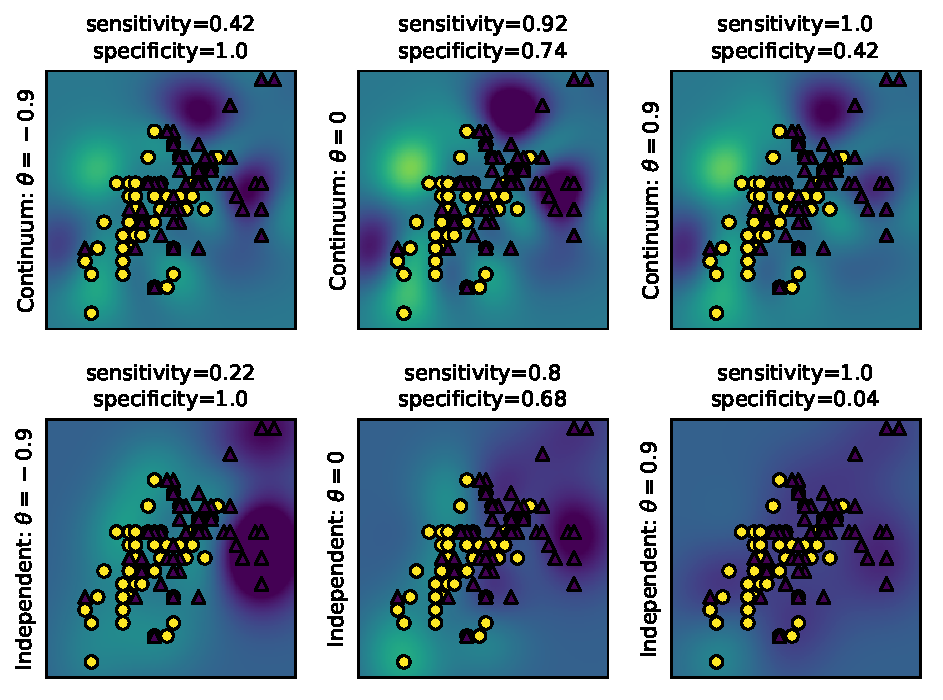
\includegraphics[angle=-90,width=\linewidth]{src/fig/autogen/icsl_vs.pdf}%
%   }
% %}
% %\fbox{
% \ffigbox[.4825\textwidth]
%   {
%     \caption{\textsc{Two-Moons} dataset}
%     \label{subfigure:csc_moons}
%   }
%   {
%     \includegraphics[angle=-90,width=\linewidth]{src/fig/autogen/icsl_vs_moons.pdf}%
%   }
% %}
% \end{subfloatrow}%
% }
% {
%     \caption{Illustration of some datasets used in \cref{table:csc_results}.
%     \label{figure:csc_datasets}}
% }
% \end{figure}%
% \textsc{Two-Moons} and \textsc{Circles} used in \cref{table:csc_results}.
